\documentclass{article}
\usepackage{geometry}
\usepackage[utf8]{inputenc}
\usepackage[polish]{babel}
\usepackage[T1]{fontenc}
\usepackage{indentfirst}
\usepackage{polski}
\usepackage{graphicx} 


\begin{document}

\title{Plantie™}
\author{Kamil Choiński, Oskar Stabla}
\maketitle

\section{Opis projektu}
Nasza koncepcja opiera się na systemie zdalnego zarządzania rośliną.
Chcemy mierzyć parametry gleby i otoczenia takie jak wilgotność, nasłonecznienie.
W zależności od odczytanych wartości przez płytkę rozwojową UNO połączoną z modułem ESP8266 będzie możliwe sterowanie pompką wody, lampą.
Mamy zamiar połączyć projekt z IT, dlatego panel sterowania będzie umieszczony na stronie internetowej.
\section{Cel}
Nasz projekt ma na celu pomoc zabieganym ludziom, którzy nie mają czasu na zajmowanie się swoją ukochaną roślinką przez swój częsty brak pobytu w domu. Wystarczy dostęp do internetu, nic więcej.
\section{Harmonogram}
\subsection{4.11}
Przeanalizowanie schematów płytki rozwojowej UNO, modułu komunikacyjnego ESP8266, czujnika wilgotności gleby, czujnika wilgotności powietrza, czujnika nasłonecznienia oraz rozwiązanie techniczne doświetlania rośliny. Stworzenie schematu elektrycznego gotowego projektu. Testowanie poprawności działania posiadanych czujników w warunkach domowych. Implementacja komunikacji z modułem ESP8266. Dopasowywanie czasów działania. 
Dokupienie brakujących komponentów gotowego projektu. 
\subsection{25.11}
Realizacja połączeń elektrycznych na płytce stykowej i ostateczne testowanie poprawności działania. Przeniesienie projektu na płytkę uniwersalną. Przygotowanie ewentualnej obudowy i realizacja montażu systemu doświetlania. Stworzenie prezentacji na zajęcia
\subsection{16.12}
Wstępna prezentacja gotowego projektu i ocena błędów.

\subsection{20.01}
Ostateczna prezentacja z poprawką błędów.


\section{Schemat blokowy}
Przedstawiony na stronie 3.
\begin{figure}
\centering
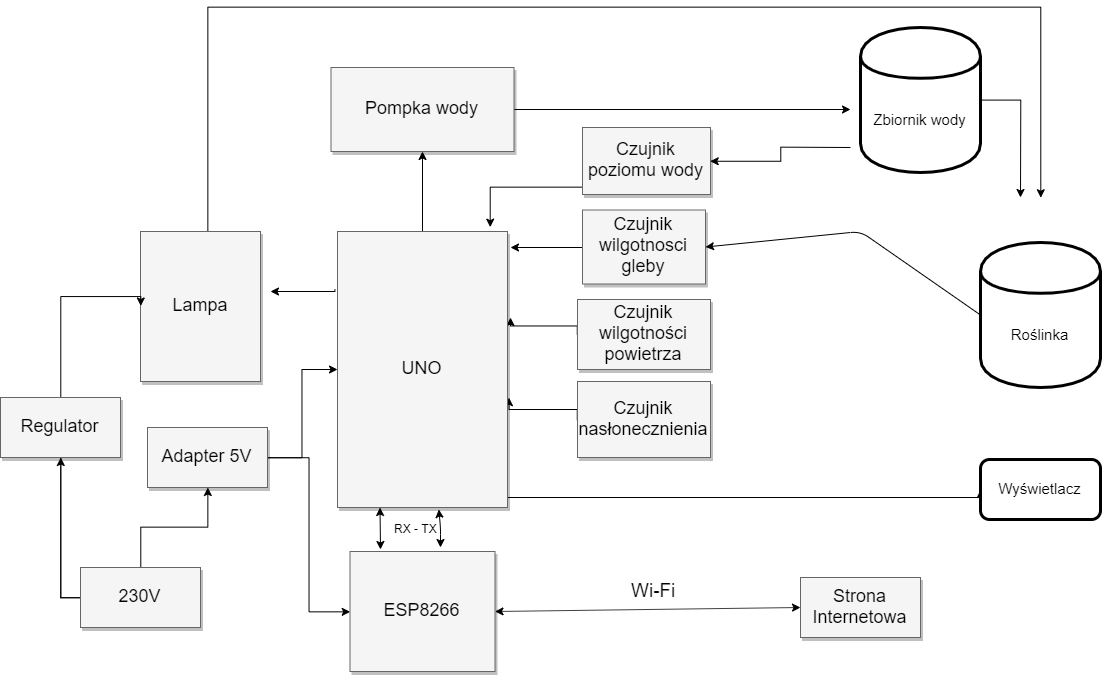
\includegraphics[scale=0.4]{schemat_blokowy}
\end{figure}


\end{document}
